\subsection{Reasoning transfer in CLEVR-CoGenT}
\label{sec:reasoning-transfer-clevr}
In the following experiments, we used CoGent-A only.
Using the question groups defined by the authors, we organized training and testing splits with the goal of measuring whether mastering reasoning for one questions group can help learning others.

\begin{figure}[htbp]
	\centering
	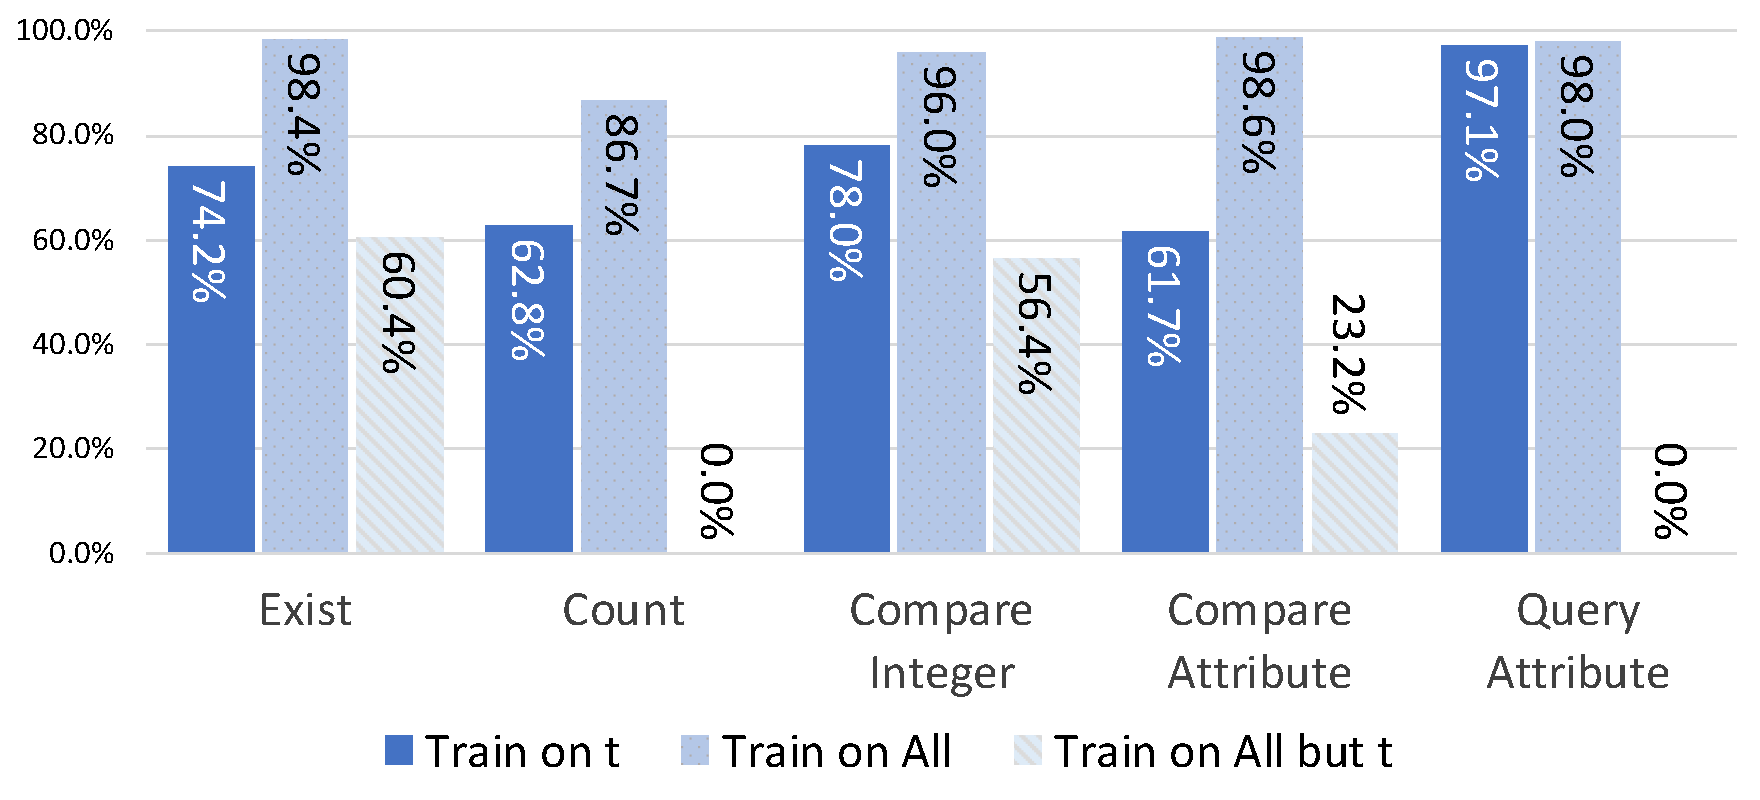
\includegraphics[width=0.8\textwidth]{../img/plots/cogent_reasoning_transfer.pdf}
	\caption{Accuracies of SAMNet when testing its reasoning transfer capabilities on the CoGenT-A variant.}
	\label{fig:cogent_reasoning_transfer}
\end{figure}

We first trained a single SAMNet instance on CoGenT-A and measured its accuracy on each of the task group $t$ separately.
Those results, indicated in \cref{fig:cogent_reasoning_transfer} as ``Train on All'', serve as baselines for the next two sets of experiments.

We next trained and tested 5 SAMNet instances, each on a single task group $t$ (``Train on t only'').
We observe significant accuracy drops (from 18 up to almost 35 points) in all task groups, except for \textit{Query Attribute}.
We hypothesize \textit{Query Attribute} requires mastering visual grounding and recognizing object attributes, as opposed to the other groups which may not enforce it.
Thus, training on \textit{Query Attribute} helps others, whereas without any training on that particular group, SAMNet struggles developing such skill.

Finally, we trained 5 SAMNet instances as follows: for each task group $t$ we trained a single instance on all tasks but $t$, and tested its performance on $t$ only.
As expected, this setup appears challenging, causing severe performance drops, with accuracy on \textit{Count} and \textit{QueryAttribute} dropping to zero.
This stems from the non-overlapping labels spaces of \textit{Count} (digits 0 to 9) and \textit{QueryAttribute} (all attributes names) with the other groups (binary ``yes'' / ``no''). Thus, the model cannot predict these labels in a zero-shot transfer.

%Besides, the zero accuracy on \textit{Count} can also be explained by the fact that it results from the need of totally different reasoning leading to the answer.
%The \textit{QueryAttribute} latter is more interesting, as when mastering e.g.  \textit{Exist} of  \textit{CompareAttribute} the model \textit{had} to develop some kind of understanding object attributes.
%Still, this result once again suggests that the model learned joint representation of object attributes and struggle with disentangling them without being explicitly trained on task facilitationg that (like the  \textit{QueryAttribute}).



% An additional set of experiments, for which results are available in the supplementary material, fine-tune the model trained on all tasks on each task $t$ respectively.
%Fine-tuning did not demonstrate a clear benefit (except for \textit{Count}, where the accuracy increased by 1.5 pt) without hurting performance on the other tasks. Nevertheless, these experiments leave open the possibility that joint training of tasks may potentially benefit from using weighted sampling towards the tail end with more emphasis on samples from less performing task groups, similar to~\cite{guo2018dynamic, kendall2018multi}.

\subsection{Reasoning transfer in COG Canonical}
\label{sec:reasoning-transfer-cog}
In order to further investigate whether reasoning transfer is effective in leveraging information gained by training a task family at a higher level of the hierarchy, we also conducted a set of experiments using the Canonical variant of COG.
The order of the performed experiments is analogical to the one in the previous section.
The first column (\cref{fig:cog_reasoning_transfer}, ``Train on All'') is taken as a reference, i.e.
we train a single SAMNet instance on all tasks and test on each of the five task groups from the task hierarchy presented in \cref{fig:task-groups}.
Please note that these results are weighted averages of the accuracies of our model on the Canonical variant tasks (\cref{fig:samnet_cog_detailed}).

\begin{figure}[htbp]
	\centering
	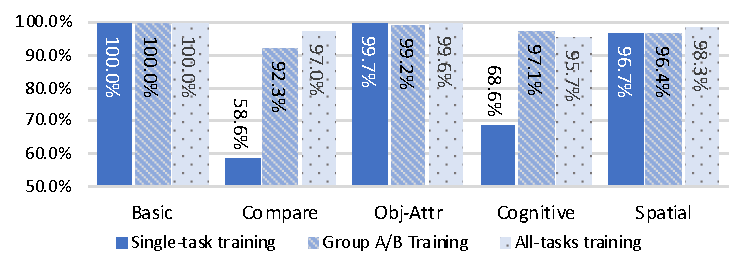
\includegraphics[width=0.8\textwidth]{../img/plots/cog_reasoning_transfer.pdf}
	\caption{Accuracies of SAMNet when testing its reasoning transfer capabilities on the Canonical variant of COG.}
	\label{fig:cog_reasoning_transfer}
\end{figure}

Next, we experimented with the ``Train on t only'' setup, i.e. training and testing each of 5 SAMNet instances on a single task group $t$ (i.e. the leaves of the proposed hierarchy).
For \textit{Basic}, \textit{Spatial} and \textit{Obj-Attr}, the accuracy is matching the reference (``Train on All''), suggesting that each group contains sufficient information for developing all necessary skills.
Therefore, models trained on these groups may not benefit from any additional training on other task groups.
However, accuracy on \textit{Compary} and \textit{Cognitive} dropped, suggesting the contrary.

Therefore, we have performed a final set of experiments (``Train on Group A/B''), where we trained two SAMNet instances: a) trained on all tasks from \textit{Group A} and tested on each task from the lowest groups (i.e. \textit{Basic}, \textit{Obj-Attr} and \textit{Compare}) separately; b) trained on all tasks from \textit{Group B} and tested separately on \textit{Spatial} and \textit{Cognitive}.
As expected, training on the other tasks from \textit{Group A} enabled the model to significantly improve on the \textit{Compare} task (from 58.6\% to 92.3\%).
A similar improvement (from 68.8\% to 97.1\%) was observed in the second experiment, when trained on \textit{Group B} and tested on \textit{Cognitive}.
Moreover, the achieved accuracy is in fact higher by 1.4 point than the one achieved when training on all tasks (95.7\%).
This suggests the model may have lacked capacity to master questions from all tasks and that training on a smaller subset allowed better performance on this subset.
Finally, we can interestingly note for \textit{Obj-Attr} and \textit{Spatial} that training on the group A/B does not appear to help. When comparing with ``Train on t only'', we observe slight accuracy drops (around 0.3-0.5 point).
Understanding this phenomenon warrants further investigations on the dependencies between the reasoning required by the particular questions and the transferred reasoning.

%With \textbf{Spatial}, we see a small improvement showing that there is some benefit due to joint training with other task families.
%To further emphasize this behavior, notice that just joining \textbf{Compare} with \textbf{Obj-Attr} and \textbf{Basic} already causes a significant accuracy jump to 92.3\%.
%In hindsight, this is not surprising, as the questions in \textbf{Compare} are composed of fragments of questions given by \textbf{Basic} and \textbf{Obj-Attr}, and therefore can leverage the reasoning strategies developed there to reason about questions in \textbf{Compare}.
% Lastly, for the \textbf{Spatial} family, we again see the benefits of joint training with all questions (68.6\% to 95.7\%) but in this case there is a slight loss incurred by including everything. As seen in the figure, just jointly training with \textbf{Spatial} alone is sufficient to get a boost in accuracy (97.1\%). To summarize, while joint training helps, one needs to determine how much of correlation is present with the other tasks.
